
\section{Linear regression}
\textbf{Linear Model}: $f(x) = \Tilde{w}^T\Tilde{x}+w_0 = w^Tx, x \in \mathbb{R}^d, y \in \mathbb{R}^n$\\
    Error Measurement: $\hat{w}= \underset{f \in w}{\text{argmin }}||y-Xw||^2$\\
    $\nabla_w||y-Xw||^2 = 2X^T(Xw-y)$, $O(nd)$, 
    \textbf{Closed Form Sol}: $\hat{w}= (X^TX)^\dagger X^Ty$, $O(nd^2)$, $n > d$: unique, $n < d$: exist 
%     via geometrical argument:
% 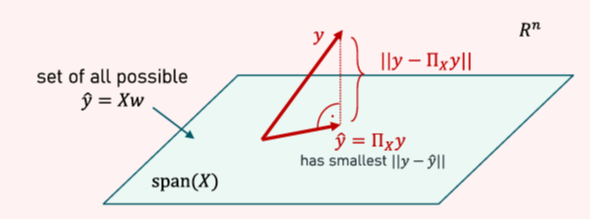
\includegraphics[width=0.6\linewidth]{pics/figure1.PNG}
    
\textbf{Huber loss }:
%\begin{equation}
    %L_{\delta}= 
    %\left\{\begin{matrix}
        % \frac{1}{2}(y - \hat{y})^{2} & if \left | (y - \hat{y})%  \right | < \delta\\
%        \delta ((y - \hat{y}) - \frac1 2 \delta) & otherwise
%   \end{matrix}\right
%\end{equation}
ignore outliers by giving less penalties
    
\begin{tabular}{c}
    $L_{\delta}(y, f(x))$ =
    $\begin{cases} 
        0.5 * (y - f(x))^2, \quad |y - f(x)| \leq \delta \\ 
        \delta * (|y - f(x)| - 0.5 * \delta),   \quad otherwise
    \end{cases}$
    \vspace{-0.3cm}
\end{tabular}
